\listfiles
\documentclass[11pt,letterpaper]{article}

% =====================
% Configuración general
% =====================
\input{config/libs.tex}
\input{config/format.tex}
\usepackage[utf8]{inputenc}
\usepackage[spanish]{babel}
\usepackage{geometry}
\usepackage{tabularx} 
\usepackage{booktabs} 
\usepackage{array}
\usepackage{hyperref}
\usepackage{float} % Debes poner esto en tu preámbulo
\geometry{a4paper, margin=2.5cm}
\newcolumntype{L}{>{\raggedright\arraybackslash}X}
\usepackage{csquotes}
\sloppy
% =====================
% Documento
% =====================
\setlength{\headheight}{14pt}
\addtolength{\topmargin}{-2pt}
\begin{document}
\renewcommand{\figurename}{Ilustración} 
{\textbf{\textcolor{azulOscuro}{INFORME PROYECTO}}}

%===========================================================
%===========================================================
% --- Tabla de Datos ---
%===========================================================
%===========================================================

{\setlength{\parskip}{0pt}
\section{Datos Generales}
}

\begin{tabularx}{\textwidth}{|>{\raggedright\arraybackslash}X|>{\raggedright\arraybackslash}X|}
\hline
Título del Informe: &  Aplicación Móvil para Optimización y Control de Entregas Logísticas - Packlead \\
\hline
Autor(a): & Carlos Hernández, Olivier Paspuel, Antonio Revilla, Frederick Tipán\\
\hline
Carrera: & Ingeniería en Software \\
\hline
Asignatura o Proyecto: & App de Logística con Geolocalización en Tiempo Real \\
\hline
Tutor o Supervisor: & Mgtr. Doris Karina Chicaiza Angamarca\\
\hline
Institución: & Universidad de las Fuerzas Armadas ESPE – Matriz Sangolquí \\
\hline
Fecha de entrega: & 10 de Febrero del 2026 \\
\hline
\end{tabularx}


%===========================================================
%===========================================================
% --- Introducción ---
%===========================================================
%===========================================================

\section{Introducción}
El presente informe expone el desarrollo de una aplicación móvil enfocada en la gestión logística y el seguimiento en tiempo real de pedidos. Este tipo de sistema surge como una alternativa para optimizar los procesos de distribución, mejorar la trazabilidad de las entregas y brindar mayor visibilidad operativa tanto a administradores como a repartidores. A través del uso de herramientas de geolocalización y monitoreo constante, se busca apoyar una toma de decisiones más eficiente dentro del entorno logístico.

El sistema creado tiene por nombre Packlead, combina herramientas modernas como Flutter para que funcione en diferentes plataformas, Firebase para manejar una base de datos que se actualiza en tiempo real, y servicios de mapas que muestran dónde están las entregas. Además, incluye librerías robustas como Riverpod y Dio para el manejo de estados y peticiones HTTP, respectivamente. Dando como resultado una mejor experiencia de desarrollo, pues se integraba bien con la arquitectura selecionada.

En lo que respecta a cómo funciona, la app deja monitorear en vivo a los repartidores, asignar y manejar los pedidos, y ver los datos de logística a través de paneles para administradores. La estructura de la app se pensó con ideas de que sea fácil de mantener y de hacer crecer, lo que ayuda a agregar mejoras más adelante y ajustarla a diferentes situaciones de trabajo. En general, esta solución que propusimos ayuda a que los procesos de distribución logística sean más eficientes, transparentes y con mejor calidad en el servicio.
\newpage

%===========================================================
%===========================================================
% --- índice de Contenidos y Figuras ---
%===========================================================
%===========================================================

\renewcommand{\contentsname}{Índice de Contenidos}
{\setlength{\parskip}{0pt}
\tableofcontents
}

\vspace{1.0cm}

\renewcommand{\listfigurename}{Índice de Ilustraciones}
{\setlength{\cftbeforefigskip}{2pt}
\listoffigures
}

\newpage

%===========================================================
%===========================================================
% --- Objetivos ---
%===========================================================
%===========================================================

\section{Objetivos}
\subsection{Objetivo General}
Desarrollar una aplicación móvil orientada a la gestión logística y seguimiento de pedidos en tiempo real, utilizando tecnologías modernas como Flutter, Firebase y servicios de geolocalización, con el propósito de optimizar la supervisión de entregas, mejorar la eficiencia operativa y facilitar la toma de decisiones dentro de los procesos logísticos.

\subsection{Objetivo Específicos}
- Diseñar la arquitectura del sistema mediante un enfoque modular y desacoplado, para garantizar escalabilidad, mantenimiento eficiente y correcta organización de los componentes.

- Implementar funcionalidades de monitoreo y gestión de pedidos en tiempo real, permitiendo la visualización de ubicaciones, estados de entrega y asignación de repartidores.

- Desarrollar un panel de control con indicadores y visualización de datos logísticos, para apoyar la supervisión operativa y la toma de decisiones dentro del proceso de distribución.

%===========================================================
%===========================================================
% --- Marco Teórico ---
%===========================================================
%===========================================================

\section{Marco Teórico}
% --- SECCIÓN 1 ---
\subsection{Desarrollo Móvil Multiplataforma}

\subsubsection{Framework Flutter}
Flutter es un framework gratuito y de código abierto que creó Google para hacer apps que se compilan de forma nativa y funcionan en varias plataformas, todo desde un solo código base \cite{FlutterDocES}. Lo principal de su idea es cambiar cómo se desarrolla software, ya que te deja armar, probar y lanzar apps para celulares, la web, computadoras de escritorio y hasta dispositivos integrados, usando la misma fuente. Esto ahorra un montón de tiempo y recursos. Básicamente, atiende a lo que se necesita hoy: llegar a los usuarios en cualquier pantalla sin el lío y el gasto de tener códigos diferentes para cada sistema operativo.

Flutter básicamente se arma con dos partes clave: un SDK, que es como un kit de herramientas para desarrollar software, y un framework que usa widgets. El SDK trae lo necesario para convertir el código en lenguaje nativo, ya sea para procesadores ARM o Intel, o incluso en JavaScript, lo que asegura que las apps corran rápido y se sientan suaves para el usuario \cite{FlutterStudyDocker}. El framework está hecho en Dart y viene con una gran colección de widgets que puedes ajustar a tu gusto, dándote control total sobre cada detalle de la interfaz. Así, es más fácil crear diseños que se adapten bien y se vean consistentes en cualquier dispositivo o plataforma. Además, una cosa genial es el \textit{"hot reload"}, que deja ver los cambios en el código casi de inmediato sin que la app pierda su estado actual, y eso acelera mucho el proceso de probar y arreglar cosas.

\subsubsection{Lenguaje Dart}
Dart es un lenguaje de programación actual y con tipos estáticos que Google inventó para crear apps que corran bien en varias plataformas. Su estructura combina una forma de escribir código clara y conocida, parecida a la de Java o C\#, con funciones más avanzadas que lo hacen perfecto para armar interfaces de usuario modernas. Como dice, “Dart es un lenguaje optimizado para aplicaciones UI, enfocado en el desarrollo en cualquier plataforma” \cite{DartWiki2024}. Y por eso, se convierte en la base principal de tecnología para el framework Flutter.

La estructura técnica de Dart permite una compilación que se adapta bien, y eso es esencial para desarrollar en varias plataformas. Puedes compilar el código Dart de antemano (AOT) a código nativo para apps móviles y de escritorio que necesitan correr rápido y eficiente, o hacerlo en el momento (JIT) para cosas como el \textit{``hot reload''} mientras estás programando \cite{DartEvolution2024}. Otra cosa importante es su sistema de tipos con \textit{sound null safety}, que evita los errores típicos de referencias nulas. Lo explican como “un sistema de tipos que garantiza que ninguna expresión cuyo tipo no admita el valor nulo pueda tenerlo” \cite{DartDocHiberus}, y esto hace que el código sea más sólido en general.

\subsubsection{Programación Asíncrona}

La programación asíncrona es algo básico en el desarrollo de apps móviles actuales con Flutter, porque deja correr tareas que podrían tardar mucho, como pedir datos por internet o acceder a bases de datos, sin trabar el hilo principal donde corre todo. Y esto es clave para que la interfaz de usuario se mantenga rápida y sin trabas, ya que "las operaciones asíncronas permiten que su programa complete el trabajo mientras espera que finalice otra operación" \cite{DartAsyncAwait}. Como Dart funciona con un solo hilo, este sistema se basa en un bucle de eventos (\textit{event loop}) y en aislamientos (\textit{isolates}) para manejar tareas al mismo tiempo, donde los hilos se comunican pasando mensajes en vez de compartir memoria directamente \cite{RedwerkAsyncFlutter}.

En Dart, la asincronía se maneja básicamente con objetos Future y las palabras clave async y await. Un \textit{Future<T>} es como una promesa de un valor de tipo T que va a estar listo en algún punto más adelante, y puede estar en proceso o ya terminado, ya sea con el valor correcto o con un error \cite{DartAsyncLanguage}. Gracias a async y await, puedes escribir código que lidia con estas operaciones de manera simple y clara, casi como si fuera código normal que corre en secuencia. Si marcas una función con \textit{async}, esta devuelve automáticamente un Future, y dentro de ella usas \textit{await} para detener temporalmente la ejecución hasta que el Future termine, lo que deja libre el hilo principal para hacer otras cosas mientras espera \cite{DartAsyncAwait}.

% --- SECCIÓN 2 ---
\subsection{Arquitectura de Software}

\subsubsection{Domain-Driven Design (DDD)}

Domain-Driven Design, o DDD, es un método para diseñar software que Eric Evans presentó, y se enfoca en manejar la complejidad al poner el énfasis en el corazón del dominio y su lógica. Básicamente, modela el programa para que represente de manera precisa el mundo del negocio, basado en lo que saben los expertos en esa área \cite{Evans2003DDD}. Lo principal que busca es reducir la distancia entre cómo funciona el negocio en la realidad y el código que se escribe. Para lograrlo, fomenta que los técnicos y los expertos del dominio trabajen juntos de forma creativa, y así pulan un modelo conceptual que todos compartan \cite{WikipediaDDD}. Dos elementos clave en el lado estratégico son el Lenguaje Ubicuo, que es como un vocabulario compartido que usa todo el equipo de manera consistente y que se ve reflejado directamente en el código, y los Contextos Delimitados, o Bounded Contexts, que marcan límites claros donde un modelo del dominio aplica y se mantiene coherente, para evitar confusiones \cite{NetmentorDDD}.

En el aspecto más práctico, DDD ofrece patrones para poner en marcha el núcleo del dominio. Por ejemplo, las Entidades son objetos que tienen una identidad única y que duran con el tiempo, los Objetos-Valor son inmutables y se definen por sus características, y los Agregados son grupos de entidades y objetos-valor que se tratan como una sola unidad para mantener la consistencia, con una raíz que controla el acceso \cite{Evans2003DDD}. Además, incluye otros patrones como Servicios de Dominio, Repositorios y Eventos de Dominio, que ayudan a armar un modelo completo y que exprese bien las ideas \cite{NetmentorDDD}. Este enfoque pone el dominio por encima de los detalles técnicos, y resulta especialmente útil en sistemas complicados con reglas de negocio enredadas, porque genera software que se ajusta mejor a lo que el negocio necesita, es más fácil de mantener y está listo para cambiar con el tiempo \cite{WikipediaDDD}.

\subsubsection{Gestión de Estado Reactiva}
La gestión de estado reactiva es un patrón clave en el diseño de interfaces de usuario actuales, donde la pantalla se refresca sola cada vez que cambia algo en el estado de la app. Lo principal aquí es que la vista actúa como una función que responde al estado, y sincroniza de forma eficiente la interfaz con los datos que hay debajo. Por ejemplo, usando la idea de una bombilla inteligente, "si la variable de datos (la luz ambiental) cambia, la aplicación reacciona y se actualiza automáticamente" \cite{MediumReactivity2024}. Este estilo resuelve cuestiones antiguas como tener que manejar manualmente el DOM o lidiar con desajustes entre los datos y la interfaz, y así mejora la experiencia para el usuario y hace que los desarrolladores sean más productivos \cite{DevToReactiveState}.

Dentro del mundo de Flutter, este patrón se pone en práctica con varias bibliotecas y métodos. Opciones como Provider, Riverpod y Bloc ofrecen formas de tener una sola fuente de verdad para el estado, y solo notifican y reconstruyen los widgets que dependen de una parte específica de los datos cuando esta se modifica \cite{TrioLibraries2026}. Elegir una biblioteca depende de cosas como cuán complicada sea la app, si necesita crecer bien o si prefieres un código más declarativo. En general, este enfoque es vital para armar apps en Flutter que sean fáciles de mantener y que rindan alto, porque ordena el flujo de datos de un modo predecible y simplifica encontrar y arreglar errores \cite{MediumReactivity2024}.

\subsubsection{Patrón Repositorio}

El patrón Repositorio es una capa que se coloca entre la lógica de dominio de la app y las fuentes de datos, para que no se mezclen. Lo principal es separar bien la lógica de la aplicación de cómo funcionan las bases de datos o las APIs, ofreciendo una interfaz siempre igual y limpia para acceder a los datos, y dejando el núcleo de la app sin enterarse de detalles técnicos como si es una API REST o una base local \cite{ModyoRepoPattern}. En Flutter, este patrón va en la capa de datos y se encarga de aislar los modelos del dominio de los orígenes reales, convirtiendo los DTOs en entidades validadas y bien tipadas que la capa de dominio puede usar sin problemas \cite{MediumCleanArchRepo}.

Para implementarlo, primero defines un contrato abstracto con una interfaz o clase abstracta donde listas las operaciones disponibles, y luego creas clases concretas que meten la lógica real, como llamadas HTTP o consultas a bases de datos. Esta abstracción da mucha flexibilidad, ya que puedes cambiar o combinar fuentes de datos (por ejemplo, una API remota o una base local) sin tocar la lógica de negocio ni la interfaz de usuario, y además facilita las pruebas unitarias usando repositorios simulados o fakes \cite{CodewithAndreaRepoPattern, MediumCleanArchRepo}.

% --- SECCIÓN 3 ---
\subsection{Geolocalización y Sistemas GIS}

\subsubsection{Geolocalización GPS}
La geolocalización por GPS es esencial en apps móviles para obtener coordenadas del dispositivo. En Flutter se implementa principalmente con el plugin geolocator, que abstrae las APIs nativas (FusedLocationProviderClient en Android y CLLocationManager en iOS) para obtener la última posición conocida, la actual o actualizaciones continuas \cite{PubDevGeolocator}.

Antes de usar los datos hay que solicitar permisos con Geolocator.requestPermission(), y luego llamar métodos como getCurrentPosition() \cite{ReaniSolucionesGPS}. El plugin también calcula distancias entre puntos geográficos, útil para funcionalidades de proximidad \cite{PubDevGeolocator}. Para un funcionamiento correcto se deben declarar permisos específicos en AndroidManifest.xml y en Info.plist de iOS, manejando todo de forma responsable para respetar la privacidad y garantizar fiabilidad \cite{ReaniSolucionesGPS}.

\subsubsection{Google Maps SDK}
El plugin google\_maps\_flutter es el SDK oficial de Google para meter mapas interactivos de Google Maps directamente en apps Flutter, tanto en Android, iOS como web. Se encarga solo de todo lo pesado: conectar con los servidores de Google, mostrar el mapa y responder a los toques o gestos del usuario, así que reduces un montón de trabajo para tener mapas buenos \cite{GoogleDocsMapsConfig}.

Para usarlo solo agregas la dependencia google\_maps\_flutter al pubspec.yaml y pones una clave API de Google Maps que configures para cada plataforma. Lo mejor es que puedes poner encima del mapa lo que quieras: marcadores para señalar puntos, líneas o polígonos para dibujar rutas o zonas, y mover la cámara del mapa como te dé la gana con código \cite{GoogleCodelabsMaps}. Gracias a que Google Maps cubre casi todo el planeta con actualizaciones constantes, sirve perfecto para cosas simples como mostrar una ubicación o para sistemas más avanzados como seguimiento de repartidores o rutas en tiempo real dentro de una app Flutter \cite{GoogleDocsMapsConfig}.

% \subsubsection{Bases de Datos en Tiempo Real}
% Una base de datos en tiempo real está pensada para que cualquier cambio que se haga se refleje al instante en todos los dispositivos conectados. Firebase Realtime Database es un claro ejemplo en el mundo móvil: guarda los datos en formato JSON en la nube y los sincroniza automáticamente con cada cliente que esté conectado, sin que tengas que hacer nada complicado de red o polling \cite{FirebaseDocsRTDB}. Esto facilita mucho crear apps colaborativas como chats, dashboards o seguimiento de ubicación en vivo.

% Lo mejor es que funciona bien incluso con internet malo o sin conexión: el SDK de Firebase guarda los datos localmente en el celular, así la app sigue respondiendo aunque estés offline \cite{FirebaseDocsRTDB}. Cuando vuelve la conexión, sincroniza solo lo que cambió de forma automática y resuelve conflictos con reglas que tú defines \cite{FirebaseProductRTDB}. Además, se accede directamente desde el código del móvil y se protege con reglas declarativas, lo que la hace perfecta para apps Flutter donde varios usuarios necesitan ver el mismo estado actualizado en tiempo real.

% --- SECCIÓN 4 ---
\subsection{Integración y Backend}

\subsubsection{Backend as a Service (BaaS)}
Backend as a Service (BaaS) es un modelo en la nube que les da a los desarrolladores de apps móviles un backend ya listo y manejado por otros. Así puedes dejar en manos del proveedor cosas como guardar datos, autenticar usuarios, lógica del servidor y notificaciones push, sin tener que configurar todo desde cero. Esto acelera muchísimo el desarrollo porque te saltas un montón de trabajo manual \cite{Back4appTutorial}. En Flutter hay plataformas como Firebase, Supabase y AWS Amplify que traen SDKs fáciles de integrar, así el equipo se puede enfocar solo en el frontend, la lógica de la app y la experiencia del usuario, sin preocuparse por servidores \cite{TrootechBackendGuide}.

Las ventajas más claras son que reduces un montón el tiempo para lanzar la app (time-to-market), la escalabilidad se maneja sola según crece el uso, y la seguridad suele estar bien cubierta por el proveedor. Entre las opciones más usadas, Firebase es el que más se ve en Flutter por su integración nativa, mientras que Supabase gusta por ser open source y usar PostgreSQL \cite{VoxturrBackend2026}. Es perfecto para prototipos, MVPs o apps que necesitan cosas en tiempo real, aunque para proyectos muy grandes y complejos puede limitar la personalización y te ata un poco al proveedor (vendor lock-in) \cite{TrootechBackendGuide}.

\subsubsection{APIs REST}
Las APIs REST son una forma estándar de diseñar servicios web para que una app (como una hecha en Flutter) pueda hablar con un servidor. Se apoyan en HTTP y usan sus métodos básicos: GET para leer datos, POST para crear, PUT o PATCH para actualizar y DELETE para borrar. Todo se hace sobre recursos que tienen una dirección única (URI) \cite{CodecademyRESTGuide}. En Flutter, para usar una API REST lo normal es hacer peticiones HTTP asíncronas con paquetes como http o dio, y los datos suelen ir y venir en formato JSON \cite{KrasamoBestPractices}.

Para que todo funcione bien y sea fácil de mantener, hay que manejar las operaciones asíncronas con async/await, centralizar las URLs base y los tiempos de espera, y controlar muy bien los errores y los problemas de red \cite{KrasamoBestPractices}. Además, es clave separar la lógica de red en una capa de servicios aparte, usar autenticación con tokens (como Bearer) para las partes protegidas, y crear modelos de datos tipados para que el código sea más seguro y no haya errores raros al procesar las respuestas \cite{MediumAdvancedIntegration}. De esta forma la app queda mucho más ordenada, fácil de probar y de mantener a largo plazo.

\subsubsection{Serialización JSON}
La serialización JSON es básicamente convertir objetos de Dart a texto en formato JSON (para enviar datos) y al revés (para recibirlos), y es algo esencial cuando trabajas con APIs REST o cualquier servicio web en Flutter \cite{FlutterJsonDocs}. Flutter trae la librería dart:convert para hacerlo a mano: tú mismo escribes los métodos toJson() y fromJson() en tus clases modelo. Funciona bien en proyectos chiquitos, pero cuando los modelos se ponen más complejos se vuelve un lío, fácil de equivocarte y difícil de mantener \cite{MediumJsonUnderstanding}.

Para apps medianas o grandes lo mejor es usar serialización automática con generación de código, como el paquete json\_serializable. Le pones anotaciones a tus clases y el paquete genera todo el código de serialización por ti con build\_runner. Así evitas repetir código, reduces errores (porque se detectan al compilar y no cuando la app ya está corriendo), maneja bien tipos complicados, nulos y cambios en los datos, y queda mucho más seguro y fácil de escalar en proyectos grandes \cite{PubJsonSerializable, FlutterJsonDocs}.

% --- SECCIÓN 5 ---
\subsection{Ingeniería de Software y Seguridad}

\subsubsection{Inyección de Dependencias}
La Inyección de Dependencias (DI) es un patrón que evita que una clase cree por su cuenta las cosas que necesita (sus dependencias), y en cambio las recibe desde afuera. Esto hace que el código tenga menos acoplamiento y sea más fácil de mantener. En Flutter es clave para conectar bien las capas de la app (como la vista, el viewmodel, el repositorio o los servicios) sin que todo quede revuelto \cite{FlutterDocComunicacionCapas}. Lo más común es pasar esas dependencias por el constructor de la clase, lo que simplifica un montón las pruebas unitarias (puedes meter mocks fácilmente) y te deja cambiar implementaciones sin tocar el código principal \cite{MediumDIInjector}.

Para manejar todo esto de forma organizada en Flutter se usan contenedores o localizadores de servicios, como get\_it, provider o injectable. Por ejemplo, get\_it es un localizador global y súper ligero donde registras las dependencias: como singletons (una sola instancia para toda la app), fábricas (nueva instancia cada vez que se pide) o lazy singletons (se crea solo cuando se necesita por primera vez) \cite{Q2BInyeccionDependencias}. Así centralizas toda la creación de objetos en un solo lugar, y la lógica de negocio y la UI quedan totalmente separadas de cómo se instancian las cosas.

\subsubsection{Manejo de Errores}
En Dart y Flutter, manejar bien los errores es clave para que la app no se caiga de golpe y el usuario tenga una experiencia decente sin sorpresas feas. Dart usa el clásico try-catch-finally para atrapar excepciones: con on capturas errores específicos que sabes que pueden pasar, y con catch agarras el objeto de la excepción más el StackTrace para ver qué pasó y depurar más fácil \cite{MediumManejoErroresDart}.

Flutter va un paso más allá y tiene sus propios ganchos: FlutterError.onError atrapa errores que pasan al construir o pintar widgets, y para los errores asíncronos que se escapan de ahí se configura PlatformDispatcher.instance.onError \cite{FlutterDocManejoErrores}. Lo ideal es envolver todo en runZonedGuarded para que capture cualquier excepción no manejada en la app, y luego enviar esos reportes a un servicio centralizado como Firebase Crashlytics o Sentry, así sabes rápido qué falla y lo arreglas antes de que afecte a muchos usuarios \cite{MediumArquitecturaManejoErrores}.

\subsubsection{Seguridad de Credenciales}
La seguridad de las credenciales es súper importante porque protege cosas sensibles como contraseñas, tokens de acceso o claves API. Lo primero y más básico es nunca dejar esas credenciales metidas directamente en el código fuente, porque alguien podría hacer ingeniería inversa y sacarlas fácilmente \cite{OWASPMobileTop10}. Si de verdad necesitas alguna en tiempo de compilación, lo mejor es usar variables de entorno o archivos de configuración que nunca subas al repositorio.

%===========================================================
%===========================================================
% --- Desarollo ---
%===========================================================
%===========================================================
\section{Requisitos Funcionales y No Funcionales}
\subsection{Descripción del Sistema}
La app \textbf{Packlead} es una aplicación móvil pensada para seguir los pedidos en tiempo real, sobre todo para mejorar todo lo que tiene que ver con la entrega de última milla en logística.
Está hecha con una arquitectura modular, o sea que separa bien la lógica del negocio (las reglas y procesos importantes) de la parte técnica de infraestructura. Así se maneja fácil los diferentes roles: por un lado los administradores y por otro los repartidores o dispatchers. Esta forma de organizarlo hace que el sistema sea más fácil de escalar, de mantener a largo plazo y de entender quién hace qué en la plataforma.

\subsubsection{Propósito}
El propósito principal de Packlead es ser una solución completa para manejar la logística de entregas, haciendo más fácil controlar todo lo que pasa en las operaciones y tener siempre una vista clara de los procesos. La plataforma te deja gestionar desde un solo lugar tanto los pedidos como a los repartidores, usando una interfaz pensada especialmente para el control.

Además, ofrece visibilidad en tiempo real del estado de los pedidos y de la ubicación de los repartidores, ayudando a optimizar los tiempos de entrega y a tomar decisiones rápidas en el día a día. Por último, el sistema mantiene todo sincronizado entre el servidor y los dispositivos móviles gracias a tecnologías en la nube, garantizando que la información esté siempre actualizada y consistente para todos.

\subsubsection{Alcance}
La aplicación incluye varias funcionalidades clave para manejar de forma completa los pedidos y la distribución. Entre las más importantes están:

\begin{itemize}
    \item El \textbf{Módulo administrativo}, que permite crear y gestionar a los repartidores, generar órdenes nuevas y ver indicadores clave de desempeño con gráficos fáciles de entender.
    \item El \textbf{Seguimiento geográfico}, que integra mapas interactivos para mostrar las rutas y los puntos de entrega en tiempo real.
    \item La \textbf{Gestión del ciclo de vida} de las órdenes, que controla con detalle los diferentes estados por los que pasa cada pedido, como pendiente, en camino o entregado.
    \item El \textbf{Esquema multiperfil}, que maneja la autenticación de forma diferente según el rol del usuario y adapta los flujos de trabajo a cada tipo de perfil.
\end{itemize}

\subsubsection{Límites y Exclusiones}
En su configuración actual, el sistema tiene algunas limitaciones importantes que hay que tener en cuenta al usarlo. Todo depende mucho de servicios de terceros, sobre todo de Google Maps Platform y Firebase, así que si alguno de estos falla o se cae, la app puede dejar de funcionar correctamente o interrumpirse por completo.
Además, como usa Firebase Realtime Database, necesita que el celular tenga internet todo el tiempo para actualizar las coordenadas y sincronizar la información entre el servidor y los repartidores. El seguimiento de la ubicación se basa solo en el GPS del teléfono del repartidor, por lo que la precisión puede variar dependiendo del modelo del celular o de las condiciones del momento. Por último, en la versión actual no hay integración de pasarelas de pago ni nada para manejar transacciones financieras directamente desde la plataforma.

\subsubsection{Componentes Principales}
El sistema está organizado en cuatro componentes principales que se ven bien claros en cómo está hecho técnicamente.

\begin{itemize}
    \item El primero es el \textbf{núcleo de gestión de estado}, que usa Riverpod para manejar el flujo de los datos y para que la interfaz reaccione rápido cada vez que algo cambia.
    \item El segundo es la \textbf{capa de servicios de ubicación}, que combina Geolocator para sacar las coordenadas del GPS y Google Maps para mostrar todo en un mapa de forma visual.
    \item El tercero es el \textbf{motor de comunicación}, que se apoya en librerías como Dio y Http para hacer las peticiones asíncronas a las APIs externas sin que la app se trabe.
    \item El cuarto es la \textbf{infraestructura en la nube}, basada en Firebase, que sirve como el lugar central donde se guardan las rutas en tiempo real y se sincronizan todos los datos entre el servidor y los móviles.
\end{itemize}

\subsection{Casos de Uso}
Para dejar bien claro cómo interactúan los usuarios con el sistema Packlead, se definen varios casos de uso. Estos casos explican las funciones principales que tienen los administradores y los repartidores (o dispatchers), enfocándose en las operaciones más importantes para manejar la logística, seguir los pedidos y controlar todo el proceso de entregas.

Definir estos casos de uso ayuda a organizar los requisitos funcionales del sistema, facilita analizarlo mejor y sirve de guía sólida para el diseño, la programación y las pruebas que se hagan después.

\begin{table}[H]
\centering
\caption{Matriz de Casos de Uso de Packlead}
\vspace{3mm}
\begin{tabularx}{\textwidth}{l l L}
\toprule
\textbf{Código} & \textbf{Nombre del Caso de Uso} & \textbf{Descripción Técnica} \\
\midrule
UC-01 & Autenticar Usuario & Permite a administradores y dispatchers acceder al sistema mediante validación de credenciales utilizando el módulo \texttt{auth\_provider.dart}. \\
\addlinespace
UC-02 & Registrar Pedido & El administrador ingresa los datos del pedido (cliente, teléfono, zona, fecha y ubicación), inicializándolo en estado \textit{pending}. \\
\addlinespace
UC-03 & Asignar Dispatcher & El administrador asocia un \texttt{dispatcherId} a un pedido existente para habilitar su visualización en la hoja de ruta. \\
\addlinespace
UC-04 & Gestionar Repartidores & Permite crear, editar y visualizar perfiles, así como monitorear su estado (\textit{available/inactive}). \\
\addlinespace
UC-05 & Consultar Hoja de Ruta & El dispatcher visualiza los pedidos asignados pendientes de entrega según su identificador. \\
\addlinespace
UC-06 & Actualizar Estado & El dispatcher actualiza el estado del pedido siguiendo el flujo \textit{pending $\rightarrow$ shipped $\rightarrow$ delivered}. \\
\addlinespace
UC-07 & Cambiar Disponibilidad & El dispatcher puede modificar su estado operativo para recibir o pausar asignaciones. \\
\addlinespace
UC-08 & Visualizar Seguimiento & El administrador supervisa en tiempo real o mediante historial la ubicación y progreso de las entregas. \\
\bottomrule
\end{tabularx}
\end{table}

\subsection{Reglas de Negocio}
Las reglas de negocio establecen restricciones operativas que garantizan la coherencia del proceso logístico, la integridad de los datos y la correcta aplicación de los roles dentro del sistema.

\begin{table}[H]
\centering
\caption{Reglas de Negocio del Sistema Logístico}
\vspace{3mm}
\begin{tabularx}{\textwidth}{l p{4cm} L}
\toprule
\textbf{Código} & \textbf{Regla de Negocio} & \textbf{Descripción} \\
\midrule
RN-01 & Ciclo de Vida del Pedido & Cada pedido solo puede adoptar tres estados: pendiente, en ruta y entregado, definidos mediante el \texttt{enum OrderState}. \\
RN-02 & Asignación de Roles & Segregación estricta según \texttt{UserRole} (admin, dispatcher, none). Rol \textit{none} no posee acceso operativo. \\
RN-03 & Geolocalización Obligatoria & No se permite registrar pedidos sin coordenadas válidas (latitud/longitud). \\
RN-04 & Estado de Repartidor & Repartidores en estado inactivo no son elegibles para nuevas asignaciones. \\
RN-05 & Integridad Temporal & Almacenamiento de fechas en formato ISO 8601 para interoperabilidad entre Flutter y Backend. \\
\bottomrule
\end{tabularx}
\end{table}

\subsection{Requisitos No Funcionales}
Los requisitos no funcionales definen atributos de calidad y restricciones técnicas que influyen directamente en el rendimiento, seguridad y mantenibilidad.

\begin{table}[H]
\centering
\caption{Especificación de Requisitos No Funcionales}
\vspace{3mm}
\begin{tabularx}{\textwidth}{l l L}
\toprule
\textbf{Código} & \textbf{Categoría} & \textbf{Requisito} \\
\midrule
RNF-01 & Arquitectura & Implementación reactiva basada en \textbf{Riverpod} para gestión de estado desacoplada. \\
RNF-02 & Portabilidad & Ejecución multiplataforma en Android e iOS mediante el framework \textbf{Flutter}. \\
RNF-03 & Persistencia & Integración con \textbf{Firebase} para sincronización en tiempo real y almacenamiento \textit{cloud}. \\
RNF-04 & Usabilidad / UI & Soporte dinámico para modo claro y oscuro según la configuración del SO. \\
RNF-05 & Configuración Segura & Uso de archivos \texttt{.env} y scripts para manejo de claves API, evitando \textit{hardcoding}. \\
RNF-06 & Robustez & Manejo de rutas inexistentes mediante pantalla \texttt{ScreenNotFound} para evitar cierres inesperados. \\
\bottomrule
\end{tabularx}
\end{table}

%===========================================================
%===========================================================
% --- Desarollo ---
%===========================================================
%===========================================================

\section{Desarrollo}

El proyecto se encuentra cargado en el siguiente repositorio de GitHub: 

\href{https://github.com/Saint-Roche-Microsystems/packlead.git}{\color{blue}\underline{https://github.com/Saint-Roche-Microsystems/packlead.git}}

\subsection{Estructura General del Sistema}
El proyecto Packlead está armado con una arquitectura modular, pensada por funcionalidades (screaming architecture). La idea principal es que sea fácil de escalar, que se pueda mantener de tal manera en la que los datos se sincronicen ante cambios de estado en la interfaz o de los servicios.

De esta forma logramos separar muy claro las partes: la lógica del negocio, el manejo de la data, la interfaz que ve el usuario y los servicios más técnicos. Así todo fluye de manera ordenada y sin que se arme lío en el sistema logístico. A continuación, se presentan los principales componentes estructurales del proyecto:

\begin{itemize}
    \item \textbf{lib/core:} Configuración global, modelos de datos compartidos y utilidades para mapas, variables de entorno y elementos base del sistema.
    \item \textbf{lib/features/admin:} Módulo administrativo encargado del monitoreo logístico, dashboard de indicadores y visualización en tiempo real de repartidores y pedidos.
    \item \textbf{lib/features/dispatcher:} Módulo operativo del repartidor que gestiona la captura de ubicación GPS, rutas asignadas y actualización de estados de entrega.
    \item \textbf{lib/features/orders:} Capa de datos que implementa el patrón Repository para la sincronización de pedidos con Firebase Realtime Database.
    \item \textbf{lib/navigation:} Sistema de enrutamiento que controla el flujo de la aplicación según el rol del usuario (administrador o repartidor).
    \item \textbf{lib/services:} Servicios técnicos para la integración con Firebase, APIs externas y acceso a geolocalización del dispositivo.
\end{itemize}

\begin{figure}[H]
    \centering
    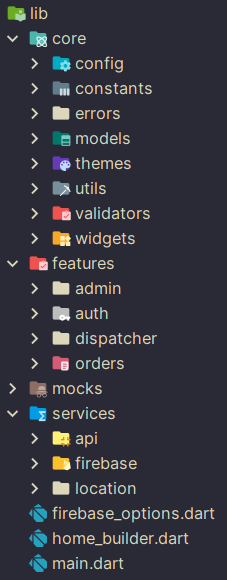
\includegraphics[width=1 \textwidth, height=15cm, keepaspectratio]{img/Estructura.png}
    \caption{Estructura}
    \label{fig:estructura1}
\end{figure}

\subsection{Sistema de Sincronización y Persistencia}
La parte que se encarga de los datos en el sistema usa el patrón Repository. Básicamente, esto sirve para que toda la lógica de cómo hablamos con la base de datos quede separada del resto de la aplicación. Así no se mezcla todo y es mucho más fácil mantener el código, hacer pruebas y después escalar el proyecto si hace falta. La clase que hace todo este trabajo es OrderRepositoryImp, que funciona como el puente entre la app y Firebase Realtime Database.

Cuando se cambia el estado de un pedido, no solo se escribe una palabra o un texto cualquiera. El sistema actualiza el estado actual y también guarda la fecha y hora exacta en que se hizo el cambio. Esto se hace con actualizaciones parciales en la base de datos, o sea, solo se toca lo que realmente cambió y no se reescribe todo el registro de una vez. Como Firebase tiene sincronización en tiempo real, cualquier modificación aparece al instante en todos los dispositivos que estén conectados: el admin, el repartidor y el cliente siempre ven la información actualizada sin tener que refrescar nada.
\begin{lstlisting}
@override
Future<void> updateOrderState(String orderId, OrderState newState) async {
  try {
    // Referencia al nodo específico del pedido en Firebase para una actualización parcial
    await _database.child('orders/$orderId').update({
      'state': newState.name,
      'updatedAt': DateTime.now().toIso8601String(),
    });
  } catch (e) {
    throw Exception('Error al actualizar el estado del pedido: $e');
  }
}
\end{lstlisting}

\subsection{Motor de Rastreo y Geolocalización Dinámica}
El sistema de rastreo es la parte más importante de la app, ya que nos permite ver en tiempo real dónde está cada repartidor. Para eso usamos el plugin Geolocator, que obtiene las coordenadas GPS del celular con la máxima precisión posible. Estas coordenadas se capturan cada cierto intervalo y las manejamos con un provider de estado reactivo que se encarga de toda la información del repartidor.

El proceso va en dos pasos: primero, la ubicación se actualiza directamente en el dispositivo para que el repartidor vea su posición actual en la interfaz sin ningún retraso. Luego, esa misma información se envía y se sincroniza con la base de datos en la nube. De esta forma, los administradores pueden ver en el mapa la ubicación exacta de cada repartidor en tiempo real.

Con este sistema se logra seguir las entregas que están en curso, ajustar rutas cuando sea necesario y mejorar la eficiencia general sin tener que estar preguntando manualmente todo el tiempo dónde se encuentra cada persona.
\begin{lstlisting}
Future<void> updateCurrentLocation() async {
  // Obtención de coordenadas actuales del GPS con alta precisión
  final position = await Geolocator.getCurrentPosition(
    desiredAccuracy: LocationAccuracy.high
  );
  
  // Actualización del estado local y notificación a la UI
  state = state.copyWith(
    currentLocation: Location(
      latitude: position.latitude,
      longitude: position.longitude,
    ),
  );
  
  // Sincronización con el repositorio para que el Admin lo vea en el mapa
  await _repository.updateLocation(state.id, state.currentLocation!);
}
\end{lstlisting}

\subsection{Dashboard de Analítica y Modelado de Datos}
El panel de administración usa una capa intermedia que se llama ViewModel. Básicamente, este ViewModel se encarga de preparar y organizar toda la información antes de mostrarla en la pantalla. En concreto, el AdminOrdersViewModel junta los datos de los pedidos, los repartidores y las ubicaciones para crear un modelo mucho más limpio y rápido que se pueda usar en gráficos, indicadores y reportes.

De esta manera, la interfaz no tiene que hacer cálculos pesados y todo fluye mejor. Así se pueden armar dashboards dinámicos que muestren los KPIs importantes, el estado actual de los pedidos y otras métricas de operación. Al final, los administradores ven en tiempo real cómo va todo el tema logístico y pueden tomar decisiones rápidas y bien informadas para que la distribución funcione más eficiente.
\begin{lstlisting}
// Cuando obtenemos un Order, construimos el AdminOrderVM (añadiendo datos extra del repartidor)
factory AdminOrdersViewModel.fromOrder(Order order, Dispatcher? dispatcher) {
  return AdminOrdersViewModel(
    id: order.id,
    clientName: order.clientName,
    clientPhoneNumber: order.clientPhoneNumber,
    location: order.location,
    address: order.address,
    state: order.state,
    zone: order.zone,
    deliveryDate: order.deliveryDate,
    createdAt: order.createdAt,
    dispatcherId: order.dispatcherId,
    dispatcherName: dispatcher?.name,
  );
}
\end{lstlisting}

\subsection{Arquitectura de Navegación por Roles}
La app tiene un sistema de navegación que depende del rol del usuario, sobre todo diferencia entre administradores y repartidores. Cuando alguien se loguea, el enrutador principal mira qué tipo de cuenta es y lo lleva directo a la pantalla que le corresponde. Así cada persona solo ve y usa las partes que realmente necesita para su trabajo, lo que hace que sea más seguro y también más cómodo de usar.

Para los administradores, la interfaz está pensada para ver todo el panorama de la logística, monitorear cómo va la operación y revisar datos y análisis. En cambio, los repartidores entran a una sección más enfocada: ver las rutas que les tocaron, seguir su entrega en tiempo real y actualizar el estado de los pedidos. De esta forma se evita que la pantalla se llene de cosas innecesarias, se reduce la confusión y nadie accede a información que no le toca ver.
\begin{lstlisting}
static Route<dynamic> generateRoute(RouteSettings settings) {
  final role = MockAuthService.currentRole;

  Route<dynamic>? route;

  if (role == UserRole.admin) {
    route = AdminRouter.generateRoute(settings);
  }

  if (role == UserRole.dispatcher) {
    route = DispatcherRouter.generateRoute(settings);
  }

  return route ?? AuthRouter.generateRoute(settings);
}
\end{lstlisting}

\subsection{Automatización de Infraestructura y Configuración}
El proyecto tiene un sistema automático para crear los archivos de configuración que necesita para conectarse a servicios externos como Firebase y Google. Todo esto lo manejan unos scripts escritos en Dart que leen las variables de entorno desde un archivo .env. Así se mantienen seguras las claves y contraseñas importantes, y se evita tener que configurar todo a mano (que siempre termina saliendo mal en algún momento).

Gracias a esta automatización, es mucho más fácil pasar el proyecto de un entorno a otro: desarrollo, pruebas o producción, sin que se arme un desastre con las configuraciones diferentes. Todo queda consistente y el despliegue se hace más rápido, más seguro y se puede repetir sin problemas cada vez que sea necesario. Esto es clave cuando la app depende tanto de servicios en la nube.
\begin{lstlisting}
Future<void> main() async {
  // Verificación de existencia del archivo de variables de entorno
  if (!File('.env').existsSync()) {
    print('Error: .env file not found');
    exit(1);
  }

  print(' Generating configuration files...\n');

  // Ejecución del proceso para generar google-services.json de forma segura
  final googleServicesResult = await Process.run(
    'dart',
    ['scripts/generate_google_services_json.dart'],
    environment: {...Platform.environment, ...envVars},
  );

  // Ejecución del proceso para generar firebase.json integrando servicios en la nube
  final firebaseJsonResult = await Process.run(
    'dart',
    ['scripts/generate_firebase_json.dart'],
    environment: {...Platform.environment, ...envVars},
  );
}
\end{lstlisting}

\subsection{Ejecución}
La aplicación inicia cargando configuraciones, conectándose a Firebase y activando los módulos principales. Posteriormente, sincroniza datos en tiempo real para monitorear pedidos, ubicaciones y estados logísticos.

\begin{figure}[H]
    \centering
    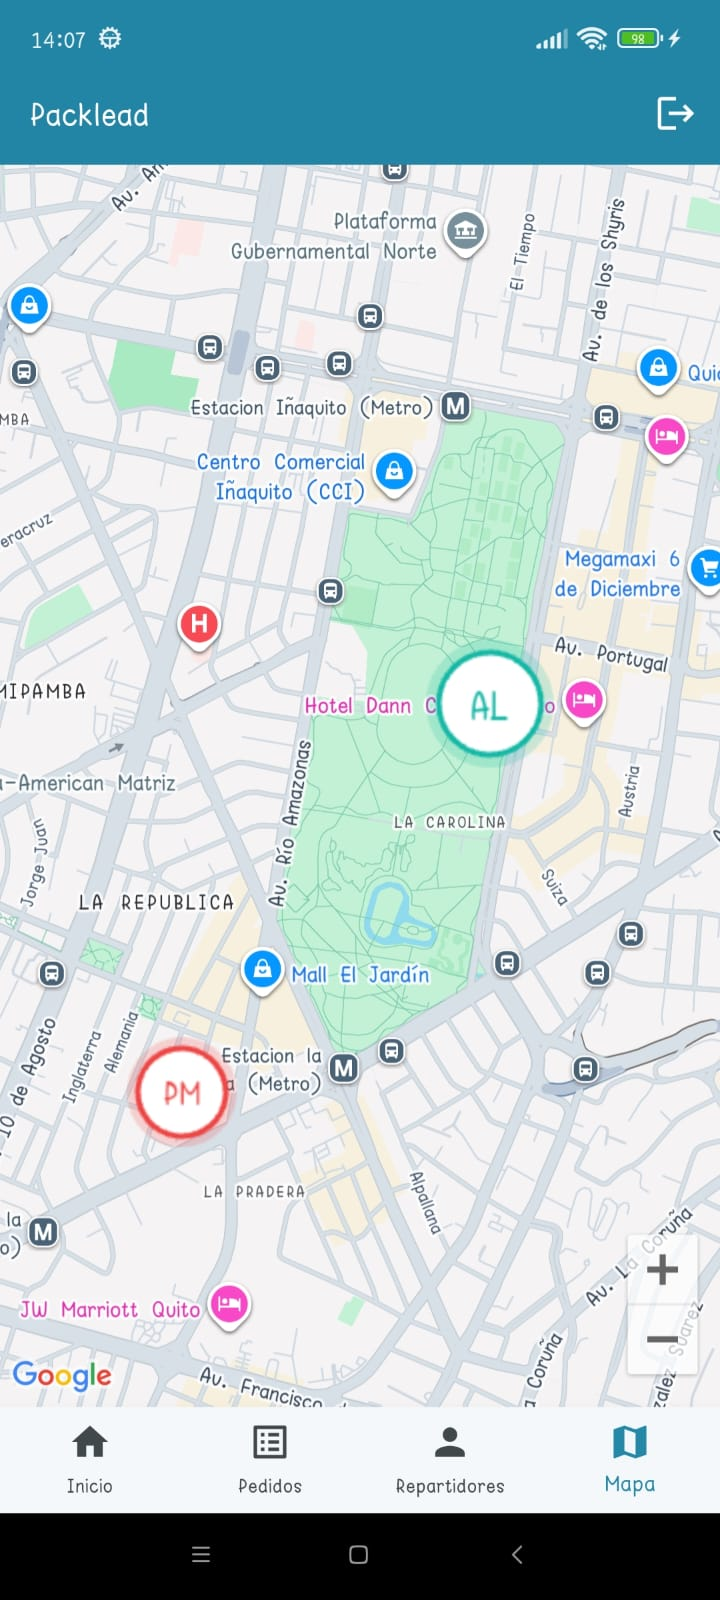
\includegraphics[width=0.8 \textwidth, height=10cm, keepaspectratio]{img/App.jpeg}
    \caption{Mapa de seguimiento en tiempo real}
    \label{fig:irt_map}
\end{figure}

\section{Pruebas}

En esta parte se explica el proceso de pruebas que hicimos para verificar que la app Packlead funcione bien, sea estable con cambios y cumpla todas las reglas de negocio que definimos. Nos enfocamos sobre todo en chequear que los datos logísticos queden intactos, que los estados de los pedidos se manejen correctamente y que los módulos del sistema se comuniquen de forma confiable entre sí.

\subsection{Estrategia y Justificación de Pruebas}
La estrategia de pruebas se centró en mantener los datos siempre consistentes y en que el sistema no se rompa cuando se agregan actualizaciones o nuevas funciones. Para lograrlo, me propuse estos objetivos principales:

\begin{itemize}
    \item \textbf{Garantizar la estabilidad del sistema:} comprobar que las actualizaciones en tiempo real que llegan por Firebase no rompan la lógica del negocio ni generen datos inconsistentes o desactualizados.
    \item \textbf{Evitar regresiones:} asegurarme de que al meter nuevas funcionalidades no se estropee nada de lo que ya funcionaba bien, sobre todo en las partes de administración y despacho.
    \item \textbf{Validar la arquitectura implementada:} verificar que el patrón Repository junto con los principios de Domain-Driven Design permitan hacer pruebas aisladas de cada parte, lo que hace el código mucho más fácil de mantener y confiable a largo plazo.
\end{itemize}

\subsection{Pruebas Unitarias (Unit Tests)}
Las pruebas unitarias se enfocaron en comprobar que la lógica de datos y los modelos funcionaran bien, sobre todo el origen de datos falso que usé para simular repartidores (\texttt{DispatcherMockDataSource}). Para hacerlas seguí el patrón \textbf{AAA (Arrange, Act, Assert)}, que ayuda a que cada prueba quede clara, ordenada y fácil de repetir.

Entre los principales escenarios evaluados se incluyen:
\begin{itemize}
    \item \textbf{Recuperación de datos:} asegurarme de que el sistema devuelva una lista correcta y válida de repartidores.
    \item \textbf{Filtrado por estado:} verificar que se pueda separar bien los repartidores disponibles de los inactivos.
    \item \textbf{Manejo de identidades:} comprobar que al pedir un repartidor por su identificador lo encuentre sin problemas, y que cuando el ID no existe devuelva lo que debe (nada o un error controlado).
    \item \textbf{Creación de registros:} confirmar que al agregar uno se le asigne automáticamente un ID con el prefijo disp- y que empiece con estado available.
    \item \textbf{Actualización y eliminación:} probar que al cambiar el estado a inactive funcione correctamente y que eliminar un registro lo saque del sistema sin dejar basura ni errores.
\end{itemize}

\subsection{Pruebas de Interfaz y Widgets (Widget Tests)}
Las pruebas de interfaz se realizaron para confirmar que el manejo de estado con Riverpod funciona correctamente con los componentes visuales de la aplicación. El enfoque estuvo en validar el comportamiento real de la interfaz desde el punto de vista de quien la usa.

Se evaluaron principalmente:
\begin{itemize}
    \item \textbf{Formularios:} se comprobó que validen bien los campos obligatorios, como las coordenadas en los pedidos, y que muestren mensajes de error claros cuando falta información o algo está incompleto.
    \item \textbf{Navegación:} se verificó que el sistema redirija al lugar correcto dependiendo del rol del usuario, ya sea administrador o repartidor.
    \item \textbf{Retroalimentación visual:} se confirmó que aparezcan notificaciones tipo Snackbar en los momentos clave, por ejemplo después de crear un repartidor con éxito, para que el usuario reciba una confirmación inmediata de que la acción salió bien.
\end{itemize}

\subsection{Pruebas de Integración y Manejo de Errores}
Las pruebas de integración se hicieron al final para comprobar que todo se conecte bien con los servicios externos y que el sistema sea sólido en general.

\begin{itemize}
    \item \textbf{Sincronización en tiempo real:} se probó que los datos entre Firebase Realtime Database y la interfaz de usuario siempre estén consistentes, mirando cuánto tardan en actualizarse y si responden rápido sin problemas.
    \item \textbf{Gestión de excepciones:} se verificó que cuando algo falla, la app muestre pantallas claras de error (como la de ScreenNotFound) y controle bien los problemas al cargar órdenes, para que no se cierre de golpe ni deje al usuario colgado.
\end{itemize}

\subsection{Ejecución de Pruebas}
\begin{figure}[H]
    \centering
    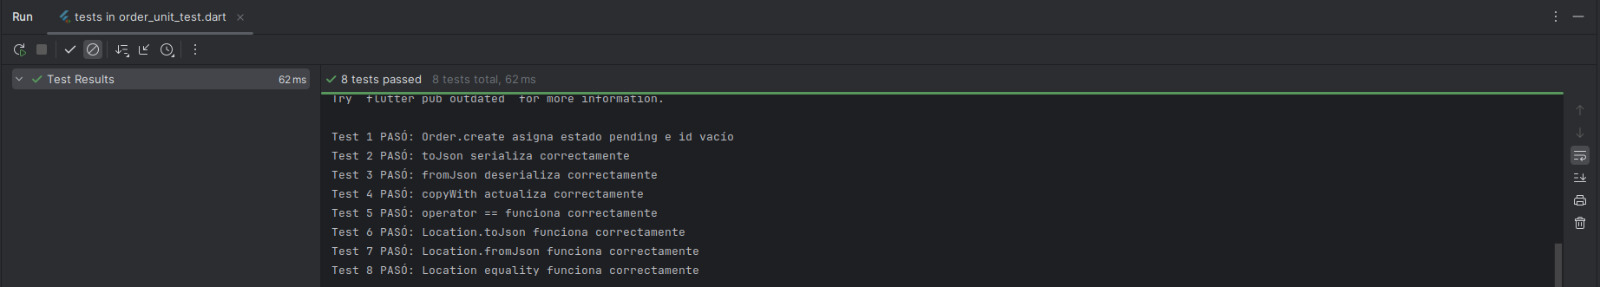
\includegraphics[width=0.8 \textwidth, height=10cm, keepaspectratio]{img/Test1.jpeg}
    \caption{Ejecución de pruebas unitarias}
    \label{fig:estructura1}
\end{figure}



%===========================================================
%===========================================================
% --- Conclusiones y Recomendaciones ---
%===========================================================
%===========================================================

\section{Conclusiones y Recomendaciones}
\subsection{Conclusiones}
\begin{itemize}
    \item La arquitectura modular que usamos en el proyecto nos permitió dividir todo bien claro. La lógica del negocio va por un lado, el manejo de los datos por otro y la interfaz queda separada. Gracias a eso mantener el sistema resulta mucho más fácil, se cometen menos errores porque las partes no se interfieren entre sí y si más adelante hay que crecer o agregar funcionalidades nuevas se puede hacer sin tocar ni romper lo que ya está funcionando.
    
    \item El uso de Firebase Realtime Database combinado con el patrón Repository nos permitió sincronizar de forma rápida y sin fallos los pedidos, sus estados y las ubicaciones. Gracias a eso tanto los administradores como los repartidores siempre trabajan con la información más reciente y actualizada en tiempo real.

    \item La integración del sistema de geolocalización y monitoreo en vivo nos ayudó muchísimo a mejorar el control de toda la logística. Ahora se puede ver en tiempo real las rutas que siguen los repartidores, el estado actual de cada entrega y exactamente dónde está cada uno. Esto hace que sea mucho más fácil tomar decisiones operativas rápidas y acertadas para que todo funcione mejor.
\end{itemize}

\subsection{Recomendaciones}
\begin{itemize}
    \item Hay que seguir mejorando la arquitectura modular del proyecto. Para eso, lo ideal es ir agregando pruebas automatizadas y también una buena documentación técnica. De esta forma se mantiene todo más estable, se evitan problemas inesperados y cuando toque hacer mejoras o agregar cosas nuevas en el futuro, va a ser mucho más fácil y rápido.

    \item Se recomienda optimizar cómo se maneja la data en tiempo real. Para eso, lo mejor es monitorear bien el rendimiento, controlar que las sincronizaciones vayan fluidas y ver si se pueden mejorar las actualizaciones para que sean más eficientes. Así se evita que la información se vuelva inconsistente entre los dispositivos.
    
    \item Se sugiere ampliar las partes de análisis y visualización de la app, agregando más KPIs, reportes detallados y métricas relacionadas con la logística. De esta forma se ayuda a planificar mejor las operaciones y los administradores pueden tomar decisiones con información más clara y completa, en lugar de ir a ciegas.
\end{itemize}

%===========================================================
%===========================================================
% --- Referencias Bibliográficas ---
%===========================================================
%===========================================================

\newpage
\section{Referencias Bibliográficas}
\printbibliography[heading=none]

%===========================================================
%===========================================================
% --- Anexos ---
%===========================================================
%===========================================================

\newpage
\clearpage
\section{Anexos}

\subsection{Pantallas de ejecución}

\begin{figure}[H]
    \centering
    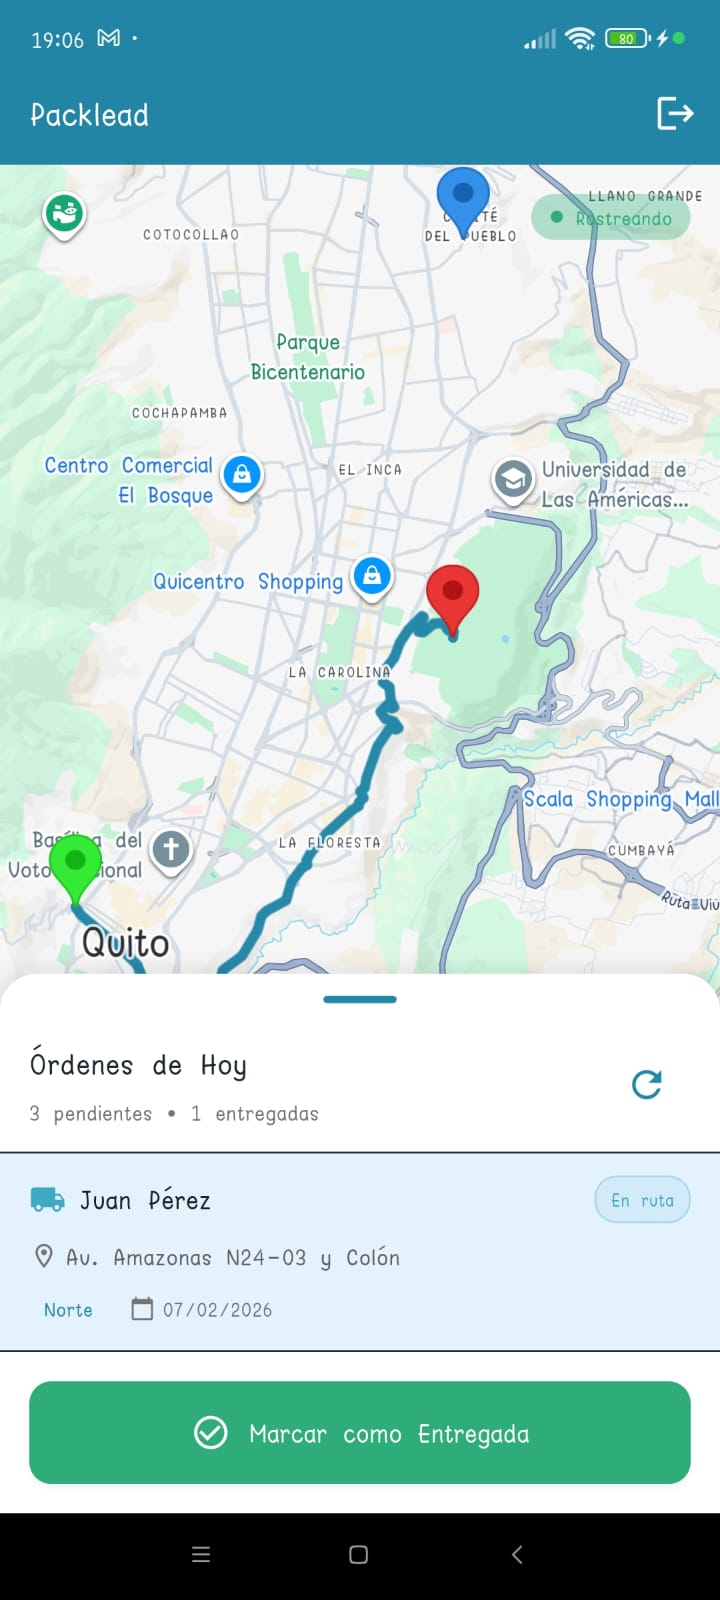
\includegraphics[width=0.6 \textwidth, height=12cm, keepaspectratio]{img/App1.jpeg}
    \caption{Mapa de repartidor en proceso de entregar una orden siguiendo una ruta}
    \label{fig:ejecucción1}
\end{figure}

\begin{figure}[H]
    \centering
    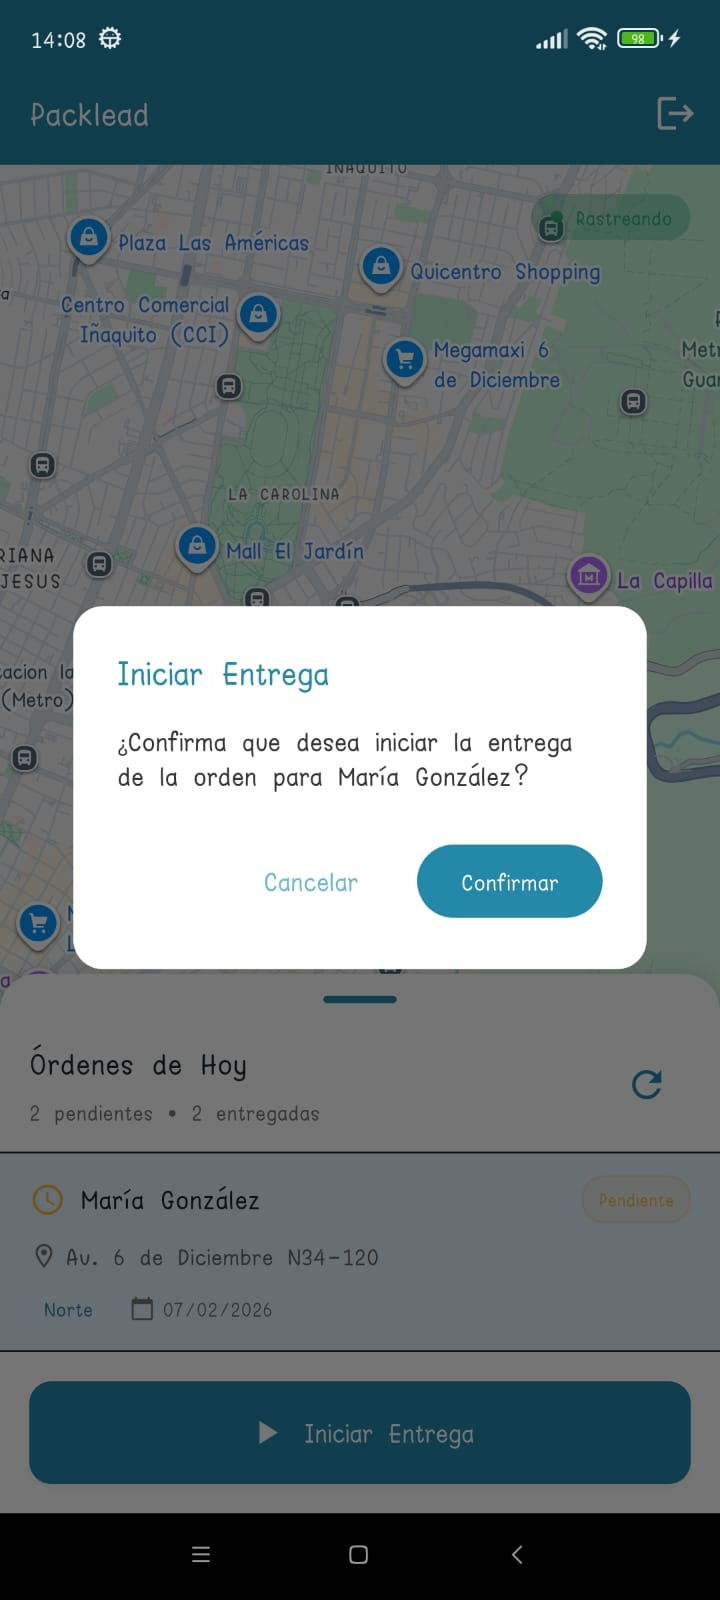
\includegraphics[width=0.6 \textwidth, height=10cm, keepaspectratio]{img/App9.jpeg}
    \caption{Mapa de repartidor confirmando el inicio de una ruta para una orden}
    \label{fig:ejecucción2}
\end{figure}

\begin{figure}[H]
    \centering
    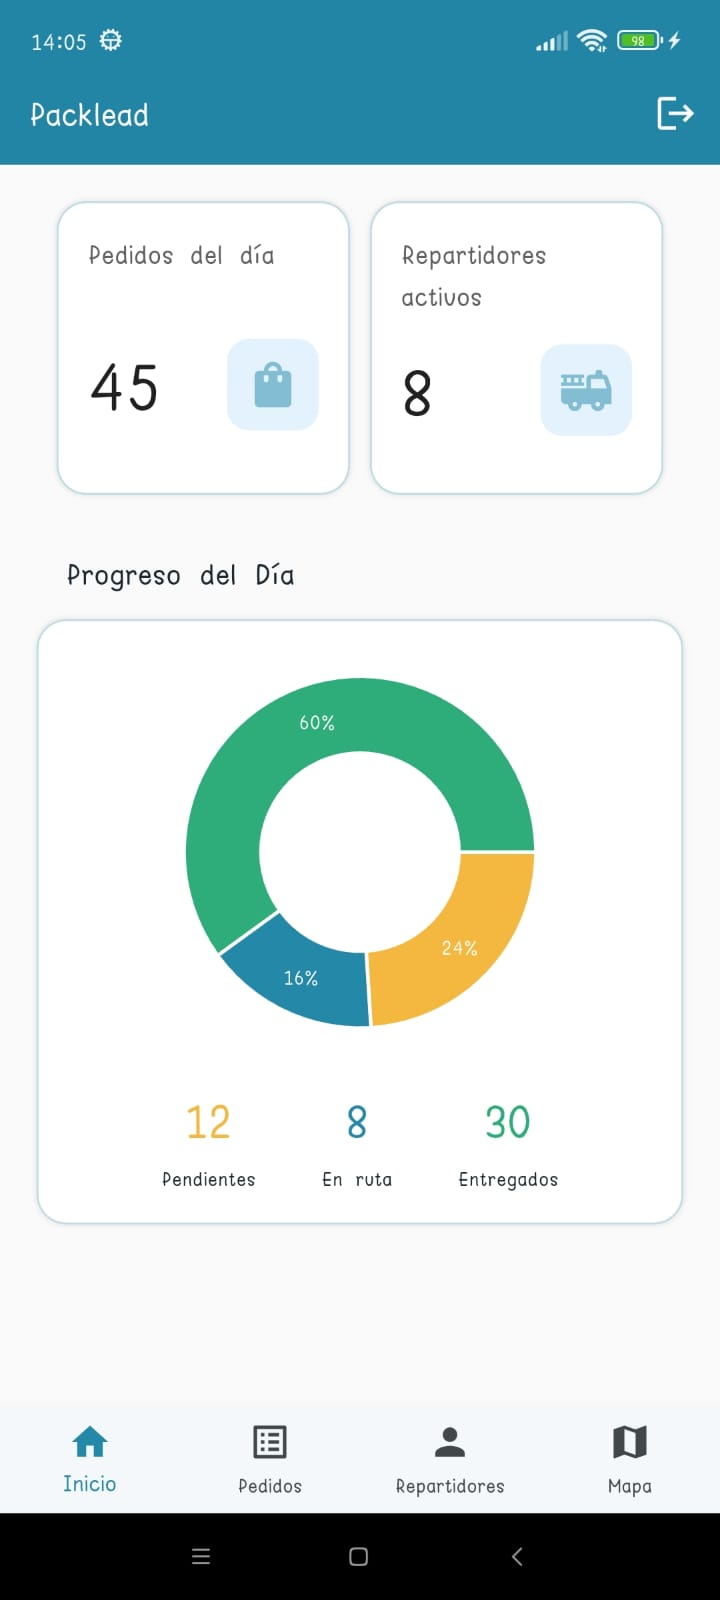
\includegraphics[width=0.6 \textwidth, height=10cm, keepaspectratio]{img/App2.jpeg}
    \caption{Dashboard del administrador para ver el resumen de las órdenes del día}
    \label{fig:ejecucción3}
\end{figure}

\begin{figure}[H]
    \centering
    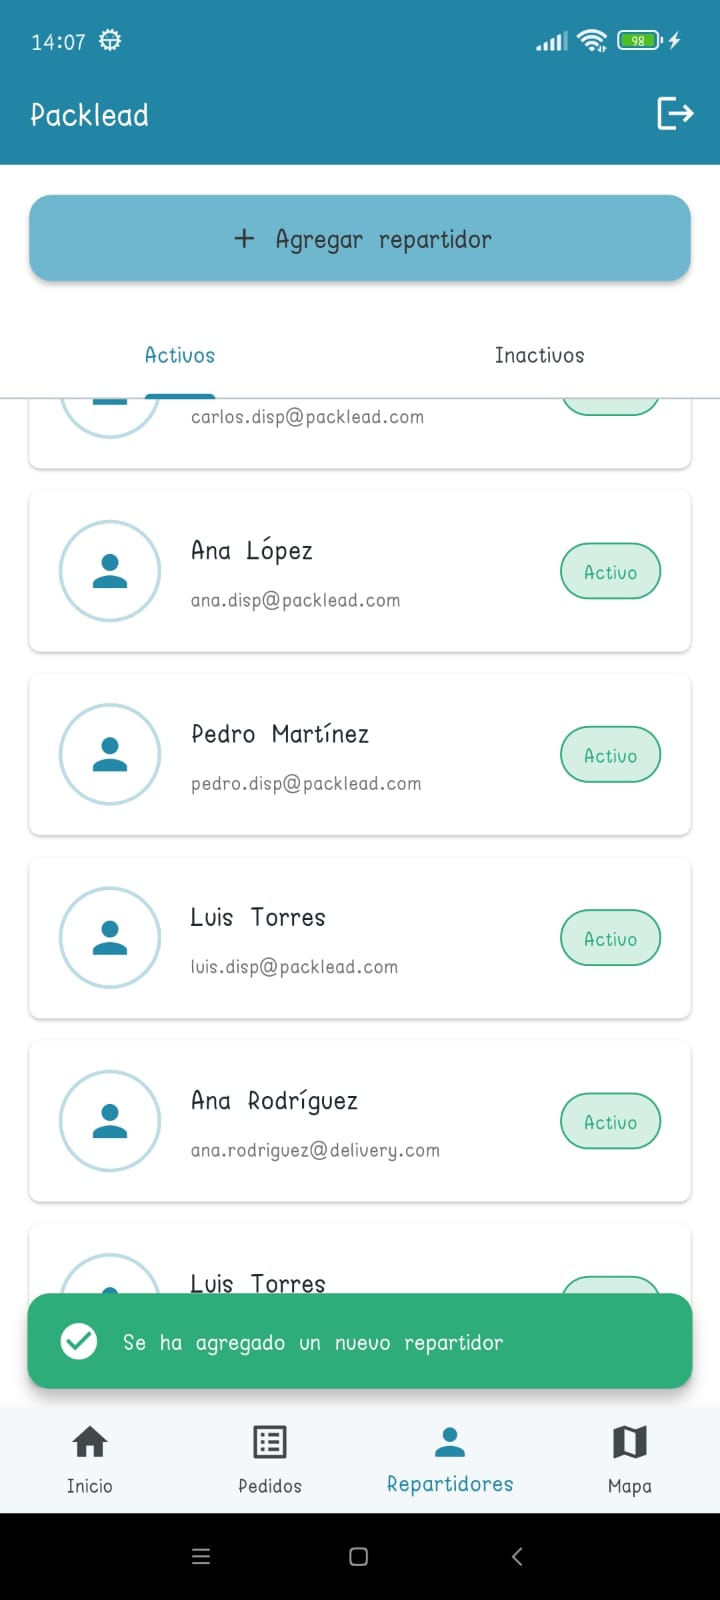
\includegraphics[width=0.6 \textwidth, height=10cm, keepaspectratio]{img/App8.jpeg}
    \caption{Snackbar de éxito mostrando que el repartidor se creó correctamente}
    \label{fig:ejecucción4}
\end{figure}

\begin{figure}[H]
    \centering
    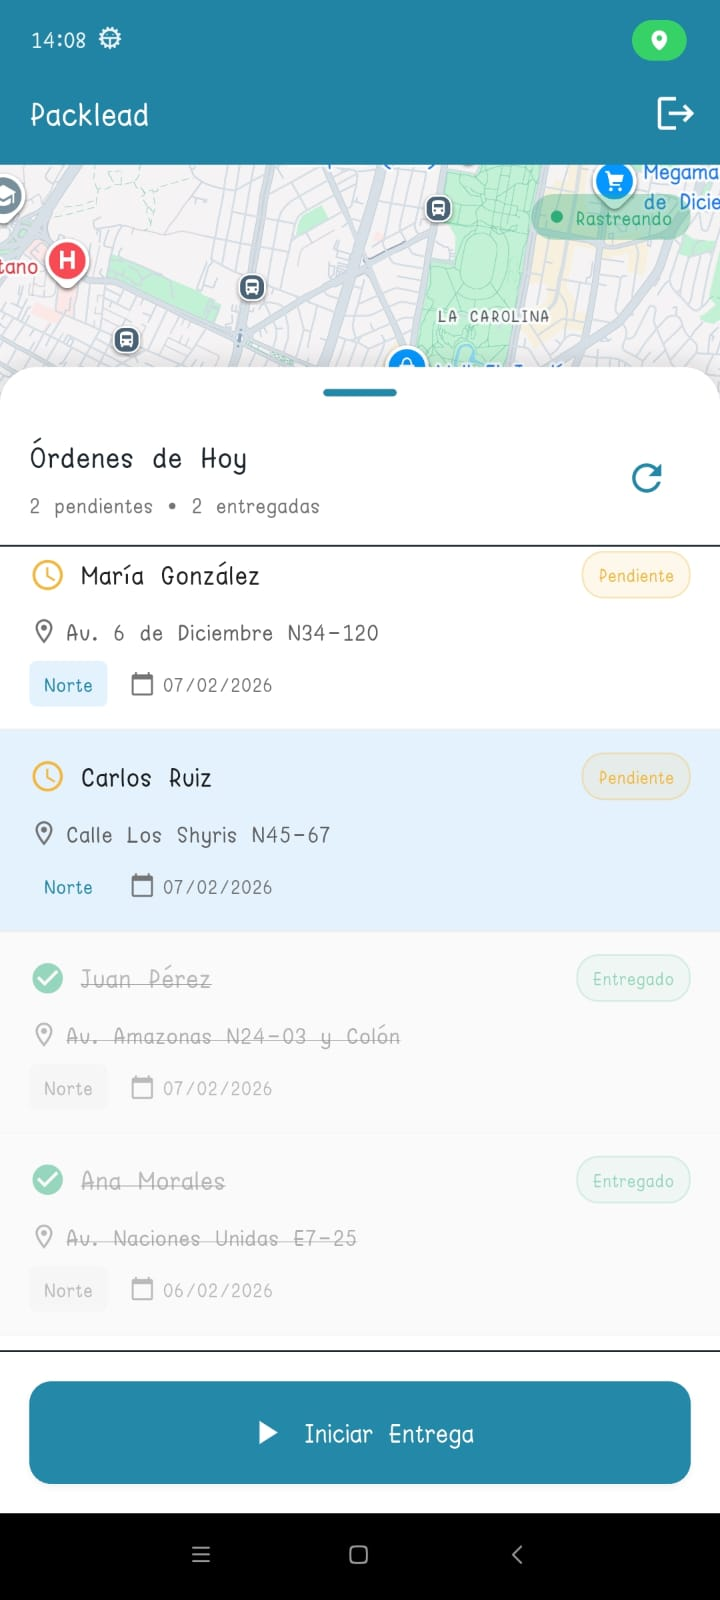
\includegraphics[width=0.6 \textwidth, height=10cm, keepaspectratio]{img/App7.jpeg}
    \caption{Lista extendida de todas las órdenes asignadas a un repartidor}
    \label{fig:ejecucción5}
\end{figure}

\subsection{Manejo de errores}

\begin{figure}[H]
    \centering
    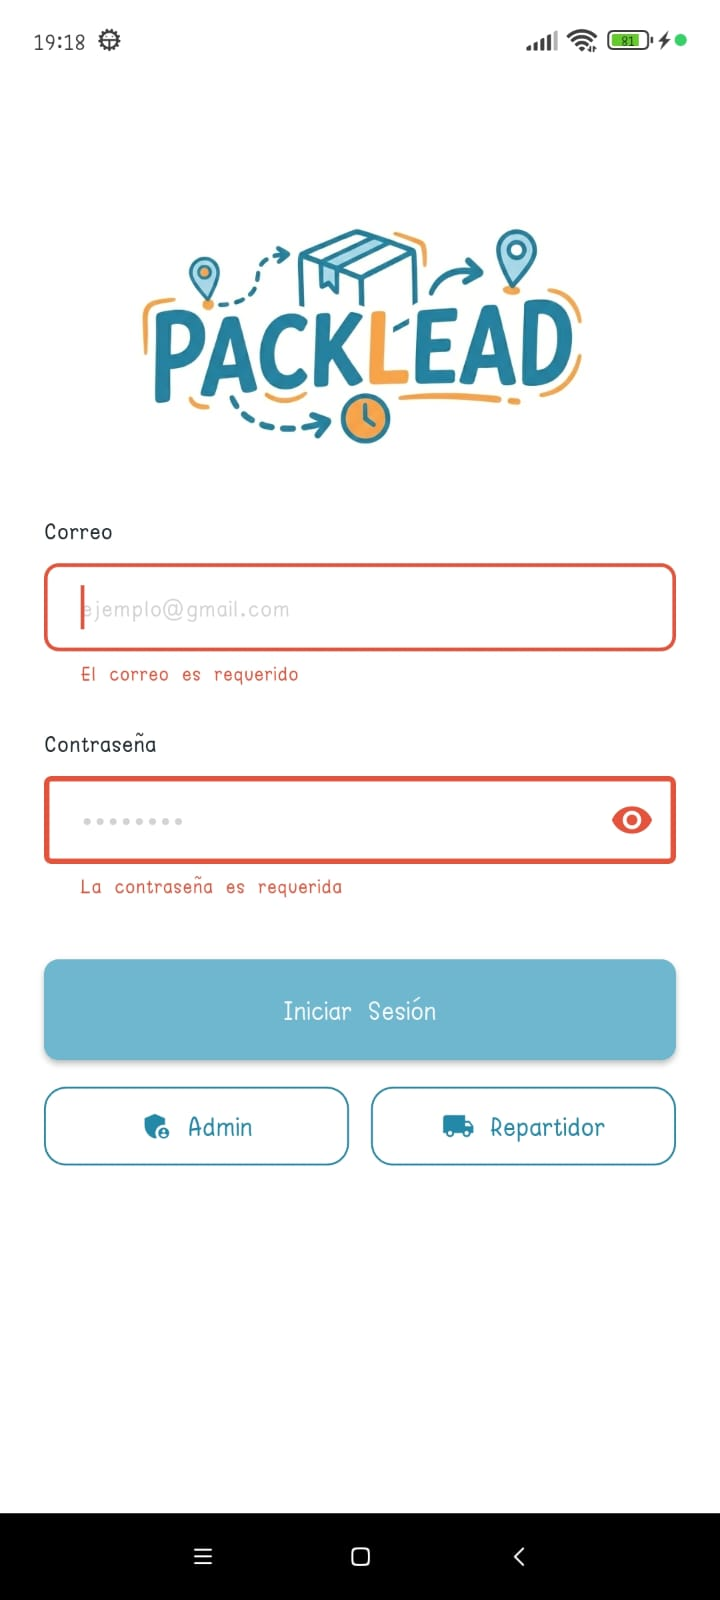
\includegraphics[width=0.6 \textwidth, height=10cm, keepaspectratio]{img/Err1.jpeg}
    \caption{Inicio de credenciales requerido en login}
    \label{fig:error1}
\end{figure}

\begin{figure}[H]
    \centering
    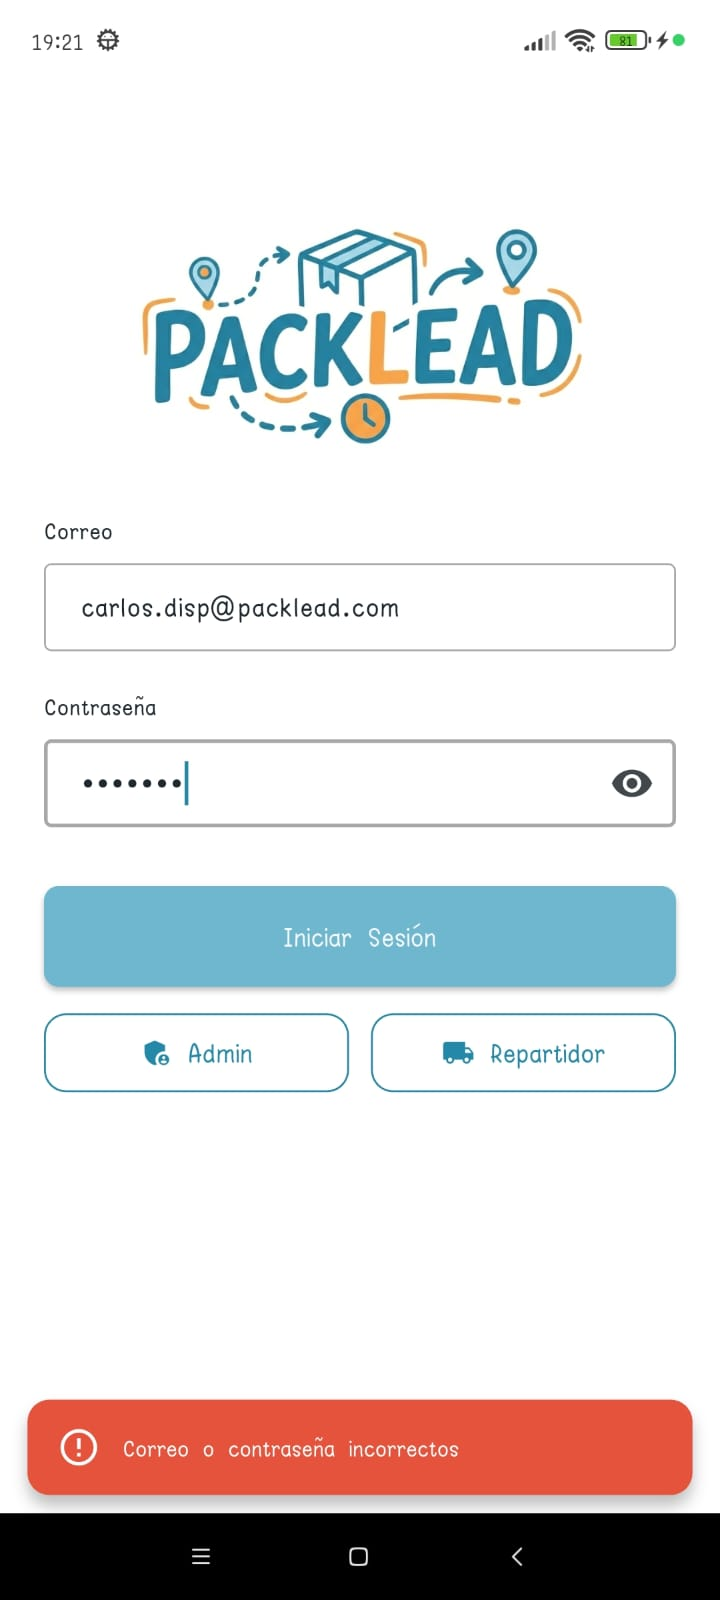
\includegraphics[width=0.6 \textwidth, height=10cm, keepaspectratio]{img/Err6.jpeg}
    \caption{Credenciales inválidas en login}
    \label{fig:error2}
\end{figure}

\begin{figure}[H]
    \centering
    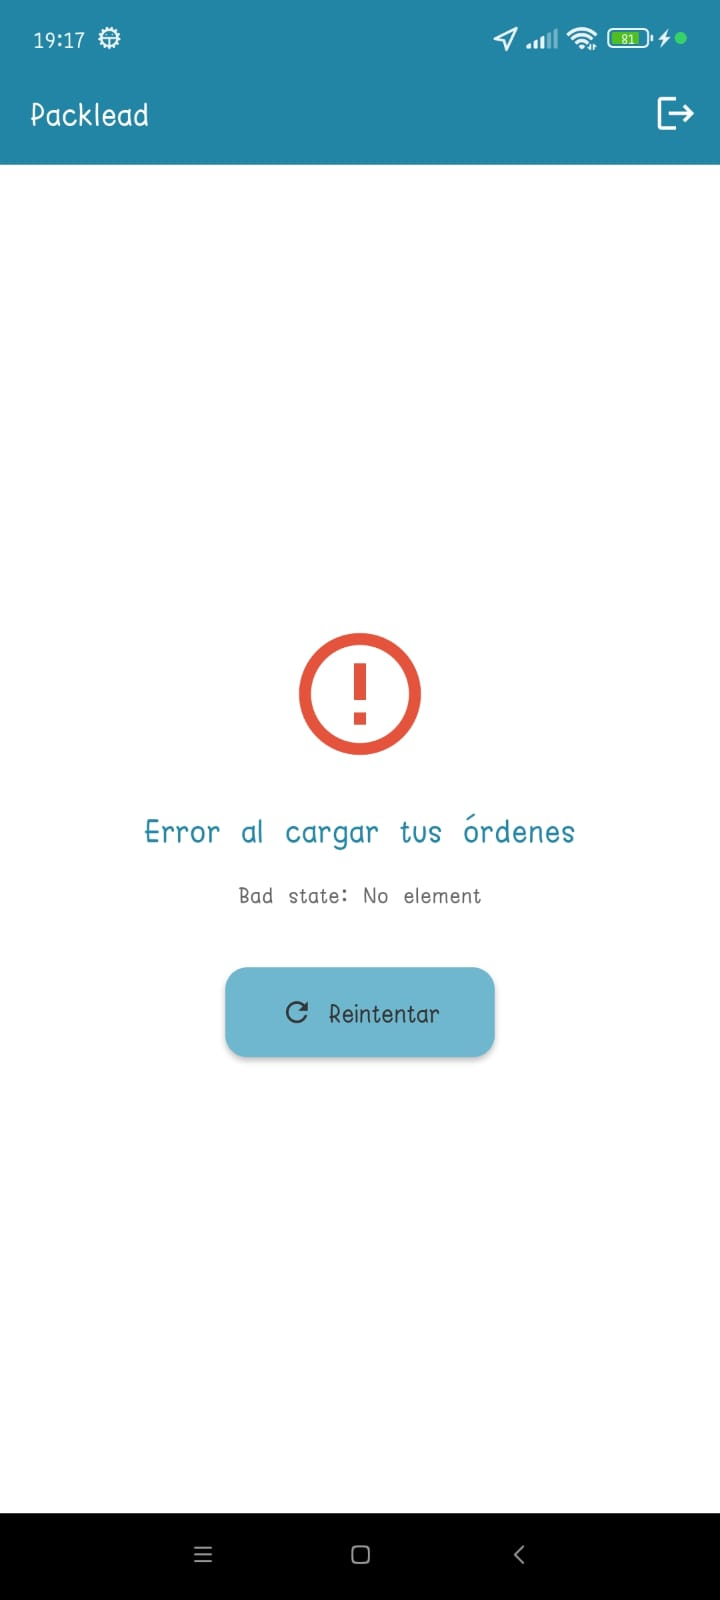
\includegraphics[width=0.6 \textwidth, height=10cm, keepaspectratio]{img/Err2.jpeg}
    \caption{Error al cargar las órdenes del repartidor en su vista principal}
    \label{fig:error3}
\end{figure}

\begin{figure}[H]
    \centering
    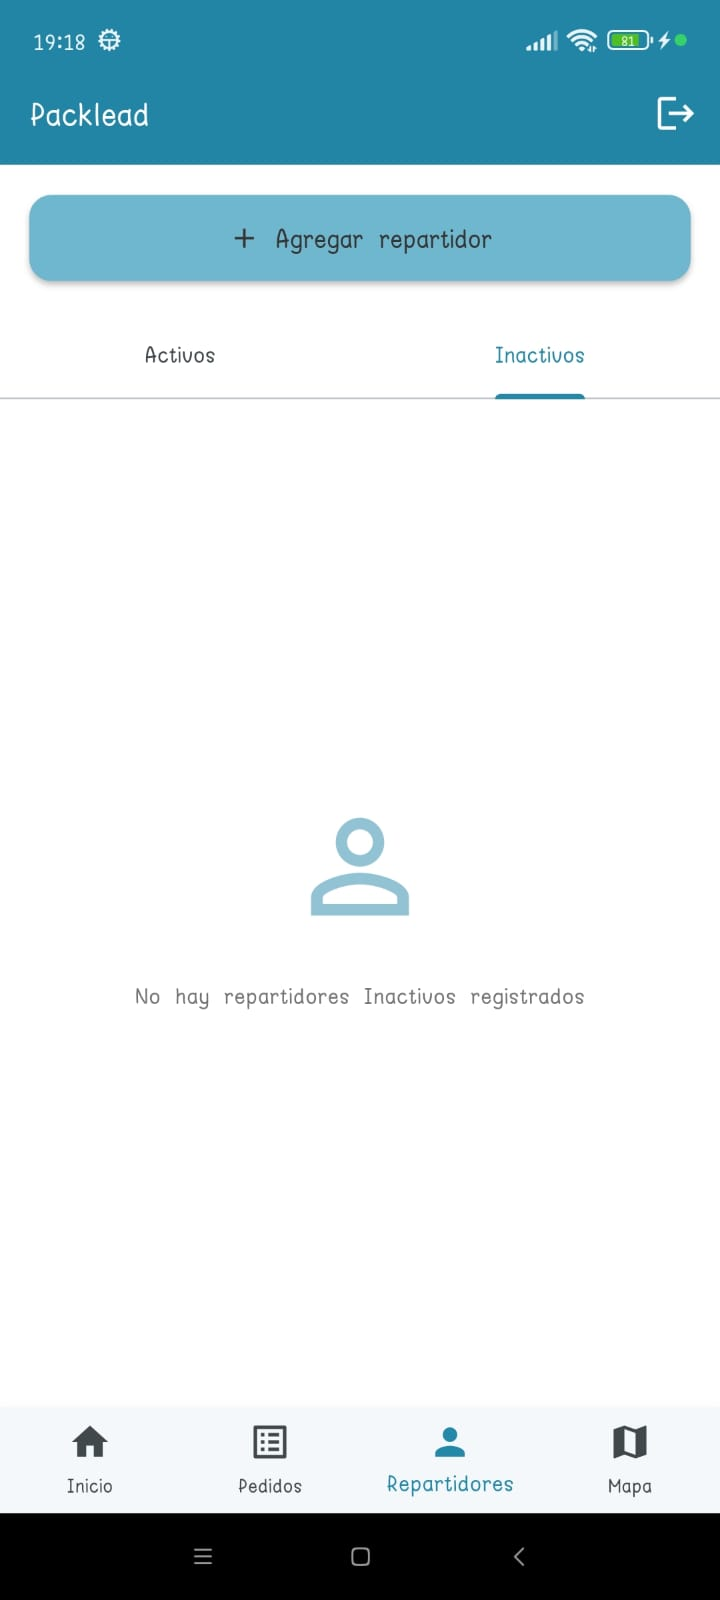
\includegraphics[width=0.6 \textwidth, height=10cm, keepaspectratio]{img/Err3.jpeg}
    \caption{Repartidores no registrados}  Ni me compilaba cuando ingresé antes
    \label{fig:error4}
\end{figure}

\begin{figure}[H]
    \centering
    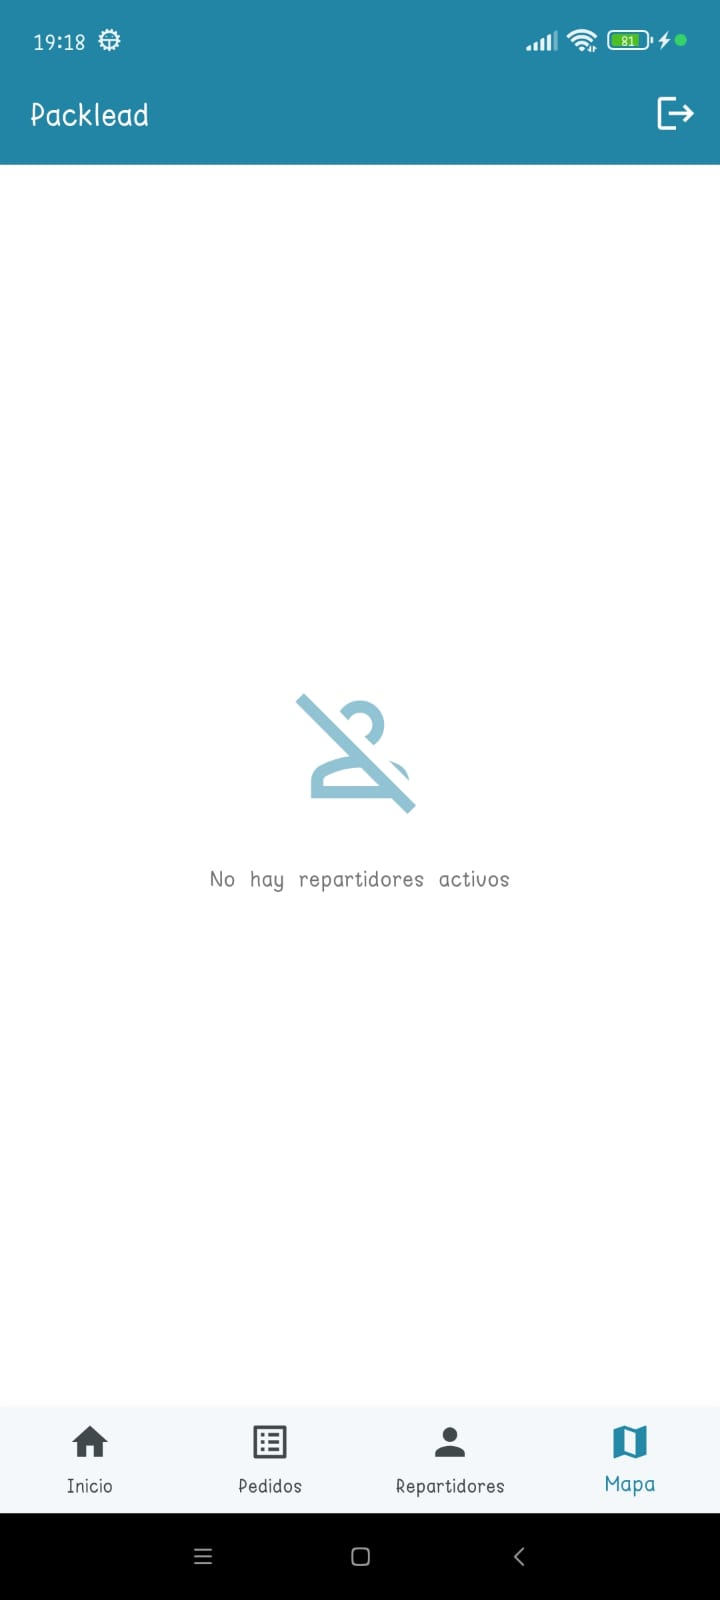
\includegraphics[width=0.6 \textwidth, height=10cm, keepaspectratio]{img/Err4.jpeg}
    \caption{Repartidores no activos para visualización de mapa en tiempo real}
    \label{fig:error5}
\end{figure}

\begin{figure}[H]
    \centering
    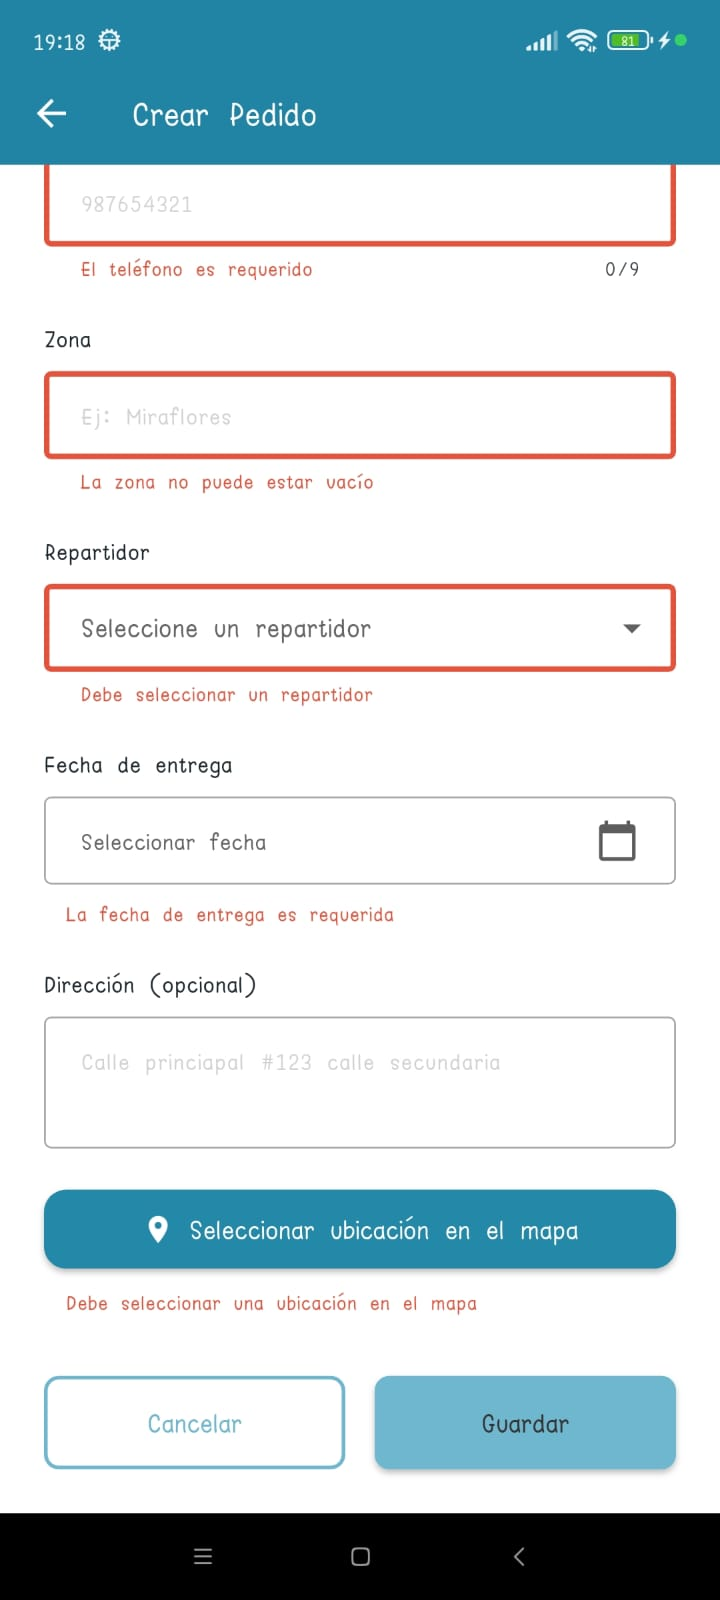
\includegraphics[width=0.6 \textwidth, height=10cm, keepaspectratio]{img/Err5.jpeg}
    \caption{Campos incompletos en formulario para agregar orden}
    \label{fig:error6}
\end{figure}

\end{document}
